% !TeX root = ../main.tex


\chapter{相关背景知识及理论基础}

\section{引言}

本章首先介绍卷积神经网络的架构,工作原理和应用。其次,介绍了本文实验中所涉及到的神经网络架构,数据集,和常用的深度学习框架。最后,对近期在优化神经网络模型存储和计算的相关工作进行综述。

\section{卷积神经网络}
卷积神经网络被广泛应用于各类机器视觉任务,如目标识别、图片分类、姿态捕捉、图片标记等。其基本主要的基本架构为卷积层+池化层+全连接层,最主要的核心运算有卷积、池化、relu等。本节主要介绍各层的在卷积网络中的各类元素、它们具体作用和计算原理。
\subsection{输入图片}
目前主流的图片编码格式有jpeg,png等,它们均采用不同方式对raw格式的图片数据进行编码存储。但卷积神经网络无法对已经编码后jpeg和png格式的图片数据处理,因此一般来说输入到卷积神经网络的图像都是原始的raw格式,即采用RGB色彩空间或YCbCr色彩空间的矩阵作为输入数据并处理。图\ref{inputImage}(a)展示了一副卷积神经网络可处理的4x4x3RGB图像。该图像有3通道的红、绿、蓝色彩空间,图中的其中每一个数值对应图像的相应色彩通道的灰度级。通常来说灰度级被定义为256,即用8bit的空间便可以进行存储。这是图像未经任何jpeg和png编码处理前最原始的表示形式,也是卷积神经网络可以处理的图片格式。用于衡量图片实际大小的单位是像素(pixels),即对应电脑屏幕最小的显示单元。一个像素的具体值由图片矩阵中RGB三通道的值线性叠加组成。如图\ref{inputImage}(b)所示,在卷积神经网络处理图片时,会将这些RGB灰度值抽取出来,其便可以用一个三维张量来表示。在实际进行推理运算时,卷积神经网络运算的对象对应图片的张量。

\begin{figure}[ht]
	\centering
	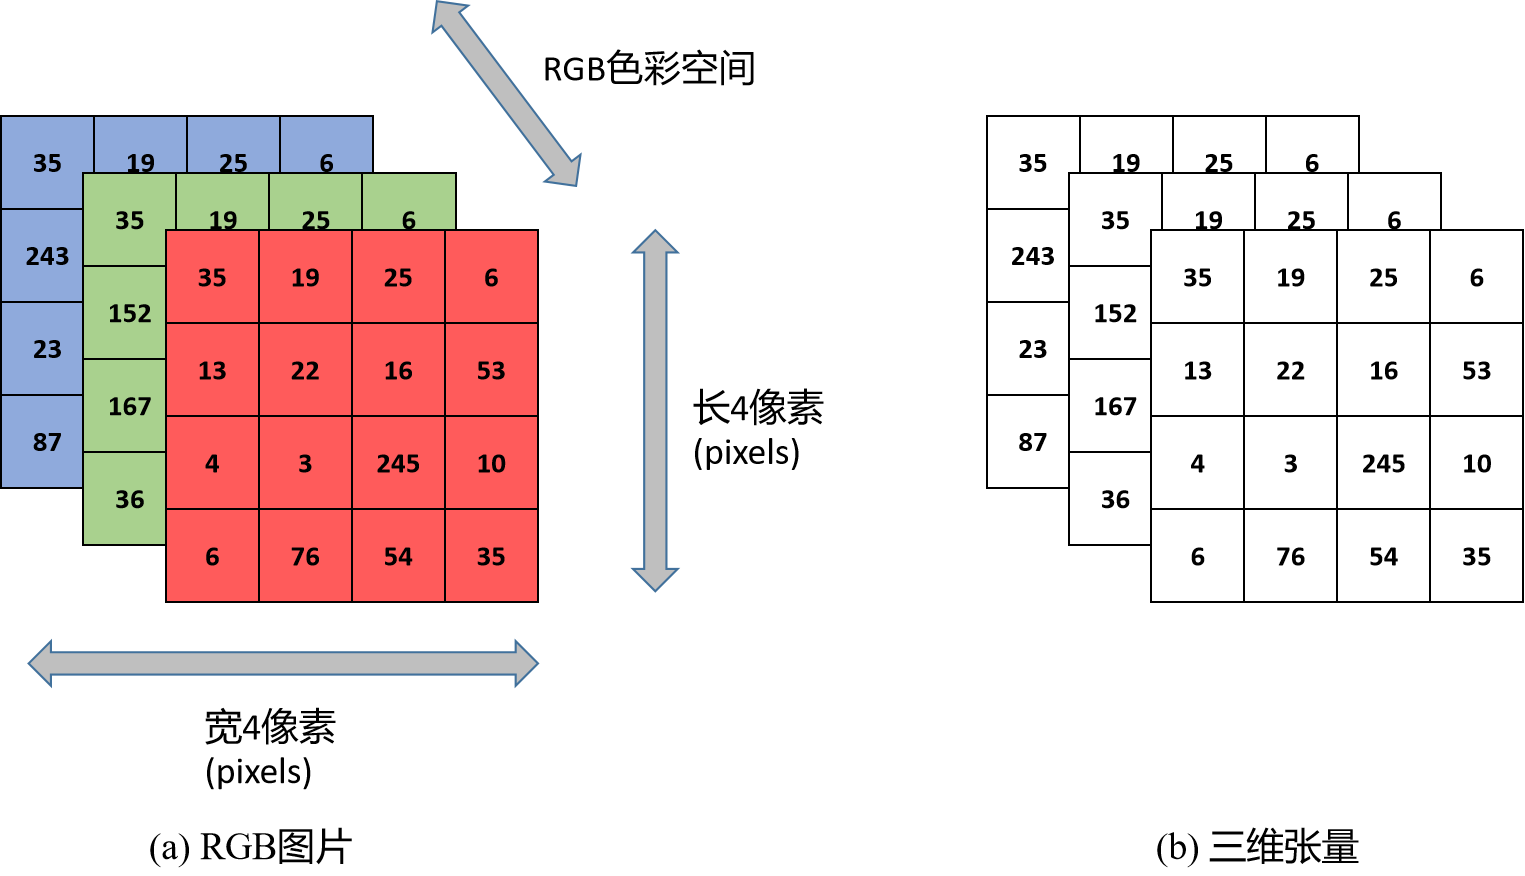
\includegraphics[width=0.8\textwidth]{figures/inputImage.png}
	\caption{4x4x3的RGB图像和其对应的张量。}
	\label{inputImage}
\end{figure}

\subsection{卷积核}
卷积核是卷积神经网络中最重要、最核心也是计算量最大的一个运算操做。卷积核会对输入图像中的一个小区域中的像素值加权求和取平均值后输出。图\ref{convOne}详细地展示了一个3x3卷积核的计算过程。首先、卷积核在进行计算时会从输入图片的左上角开始,从左往右依次移动,直到移动到图片的右下角才停止。每次移动的距离由一个数值决定,这个数值被称作\textbf{步长}。当步长等于1表示每次移动的距离是一个像素点,当步长等于2表示每次移动两个像素点。其次、卷积核在图像上每一次移动时,均会把图片中的像素值和卷积核中的数值加权求和。其计算方式如下公式\ref{conv_eq}所示:
\begin{equation}
\begin{aligned}
\label{conv_eq}
output = \sum_{i=1}^N conv_i*pixel_i
\end{aligned}
\end{equation}
其中N表示卷积核数值总数,$pixel_i$表示卷积区域中像素值,$conv_i$表示卷积特征值,ouput是该像素区域的加权输出。以图\ref{convOne}为例,该卷积核在卷积左上角的像素区域时,其卷积输出是156+156=312。
\begin{figure}[ht]
	\centering
	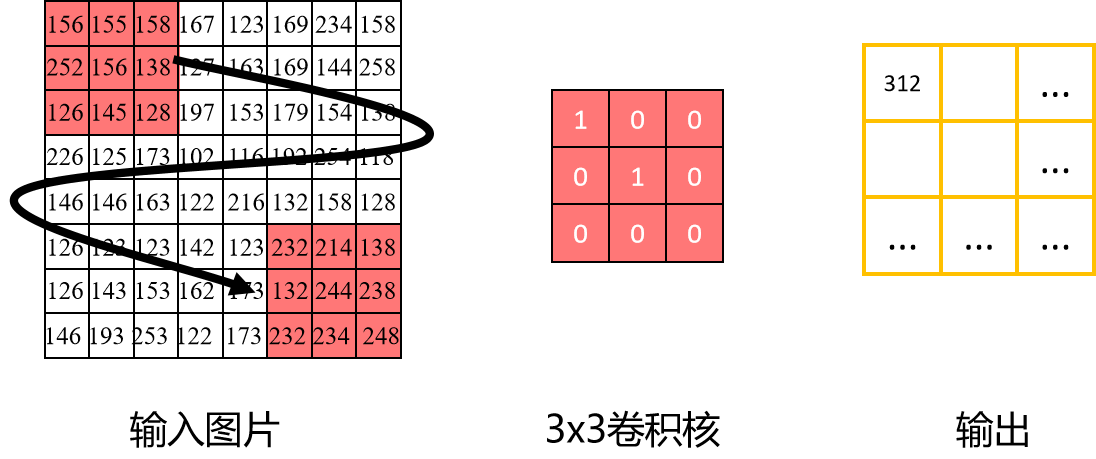
\includegraphics[width=0.8\textwidth]{figures/convOne.png}
	\caption{一个3x3卷积核的运算过程。}
	\label{convOne}
\end{figure}

由于卷积核运算中的加权求和移动计算的特点,卷积核的实际输出数目取决于卷积核的大小和卷积核移动的步长设置。如果不对图片进行任何处理,随着步长的增大,卷积核计算的输出个数会减少。这就会出现输入图片在经过卷积运算后,输出的特征图会比原来输入图片变小的现象。因此为了保证输入图片在经过卷积核运算后,其尺寸不发生变化,通常会在输入图片外围补充0,来保证卷积核输出尺寸不变,这一操做被称为\textbf{填充(padding)}。具体的来讲,存在两种填充方式:\textbf{有效填充(valid padding)}不对图像做任何填充操做,卷积运算的输出尺寸与卷积核大小保持一致;\textbf{相同填充(same padding)}根据卷积核步长的大小对图像补充0,卷积运算的输出尺寸与输入图片尺寸保持一致。图\ref{convOPS}展示了步长为1,在RGB三通道输入图像上完整的卷积计算过程。图片每一个色彩通道卷积核工作方式,同图\ref{convOne}一个卷积核计算的过程一样,三个色彩通道上的卷积核依次从左上角往右下角计算,直至将整个像素区域卷积完为止。值得注意的是,每个色彩通道外围都被补充了一圈0,这是为了保证卷积运算结束后,输出的特征图的尺寸与原输入图片尺寸保持一致。在组织形式上,三个通道的卷积核也会被组织成一个三维张量。

\begin{figure}[ht]
	\centering
	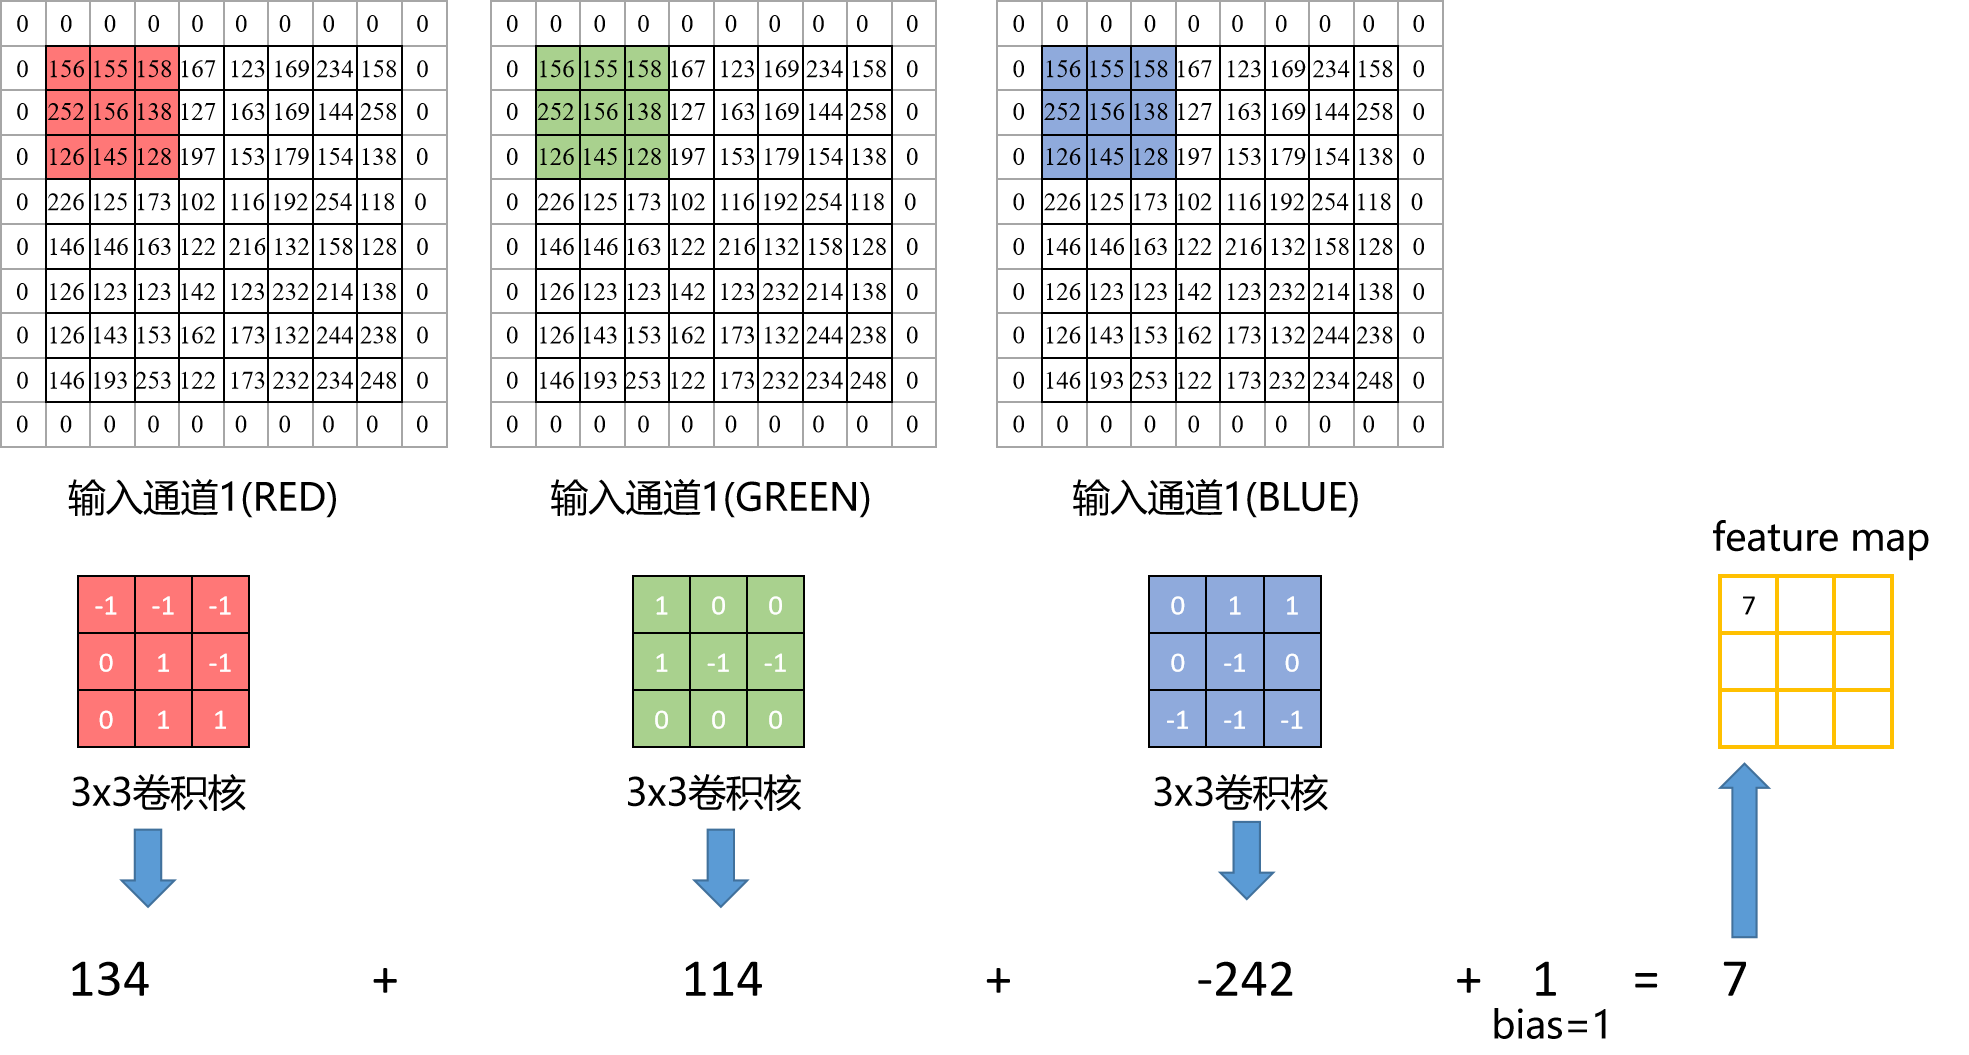
\includegraphics[width=1\textwidth]{figures/convOPS.png}
	\caption{一个3x3卷积核的运算过程。}
	\label{convOPS}
\end{figure}

卷积运算在整个卷积神经网络中目的是从输入图像中提取边缘、角度等高级特征。在卷积神经网络中,通常存在多个卷积层,这也是卷积神经网络名字的由来。在大部分卷积神经网络中,前几层负责捕获底层特征,如边缘、颜色、梯度方向等。后几层捕捉更图片中更细节的特点。卷积神经网络的学习能力随着卷积层深度的增加而提高。

\subsection{非线性激活层}
在经典的M-P神经元模型中,有一个概念是激活函数。激活函数的想法来自于生物神经元在工作时,神经元激活与否取决于某一阈值电平,即只有当其输入总和超过某个特定阈值时,神经元才被激活而发出脉冲信号,否则神经元不会发生输出信号。这个概念特化到专门处理图像数据的卷积神经网络中,激活函数被称作\textbf{非线性激活层}。类似地,在卷积神经网络中常见的非线性激活层有tanh、sigmoid和relu等。非线性激活层通常被添加在每一个卷积核层之后,用于校正线性单元,使卷积核和卷积核之间产生非线性关系,为整个卷积神经网络引入非线性关系。卷积运算本质上是一种线性运算——矩阵乘法和加法,不添加非线性激活层的话,卷积神经网络不具备学习非线性关系的能力。

从计算的角度来将,因卷积神经网络处理的数据对象是图片,非线性激活层的在进行运算操做时,是按照像素来进行运算的。与卷积核运算不同之处在于,非线性激活层对整张输入图片处理,不会移动。因此,任何特征图经过非线性激活层后,其尺寸不会发生变化。图\ref{relu}展示了特征图经过relu层后的结果。relu层会将特征图中所有小于0的数值直接抛弃,只保留大于0的像素值。通过这种方式,在为卷积神经网络添加非线性关系的同时,减少参数间相互依赖的关系,减少了过拟合的发生。并且,设置部分特征图中的数值为0,有效的减少了机器运算周期。因为机器在计算绝对0乘法时,会省去对阶、尾数运算和规格化的步骤,有效的降低了计算复杂度。其他非线性函数,如tanh或sigmoid,也可以用来代替relu,但relu的平均性能在多数情况下表现更好。

\begin{figure}[ht]
	\centering
	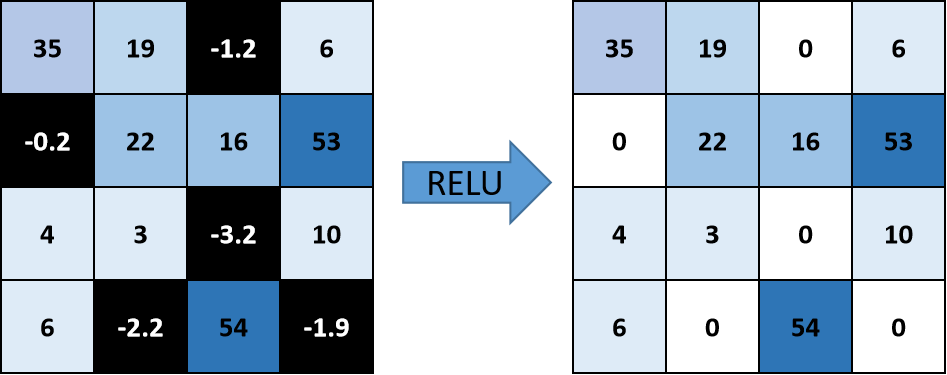
\includegraphics[width=0.8\textwidth]{figures/relu.png}
	\caption{relu层的计算方式。}
	\label{relu}
\end{figure}

\subsection{池化层}
\textbf{池化层(pooling)}也被称为\textbf{下采样(downsampling)},其主要作用是负责减少卷积运算后得到的特征图的尺寸大小,并保留重要的特征信息。在卷积神经网络计算中,使用池化层减小特征图大小有三个积极意义:1)使用池化能够有助于提取旋转和位置不变的主要特征,从而让模型有更好的训练结果。2)减小特征图的大小能够显著减少卷积神经网络计算期间的计算量和内存读写量,从而减少推理单张图片所需耗费的时间。3)池化能够有效提取出特征图中的主要特征。从类别上来讲,池化层主要有最大池化(max pooling),平均池化(Average Pooling),求和池化(Sum Pooling)等。

\begin{figure}[ht]
	\centering
	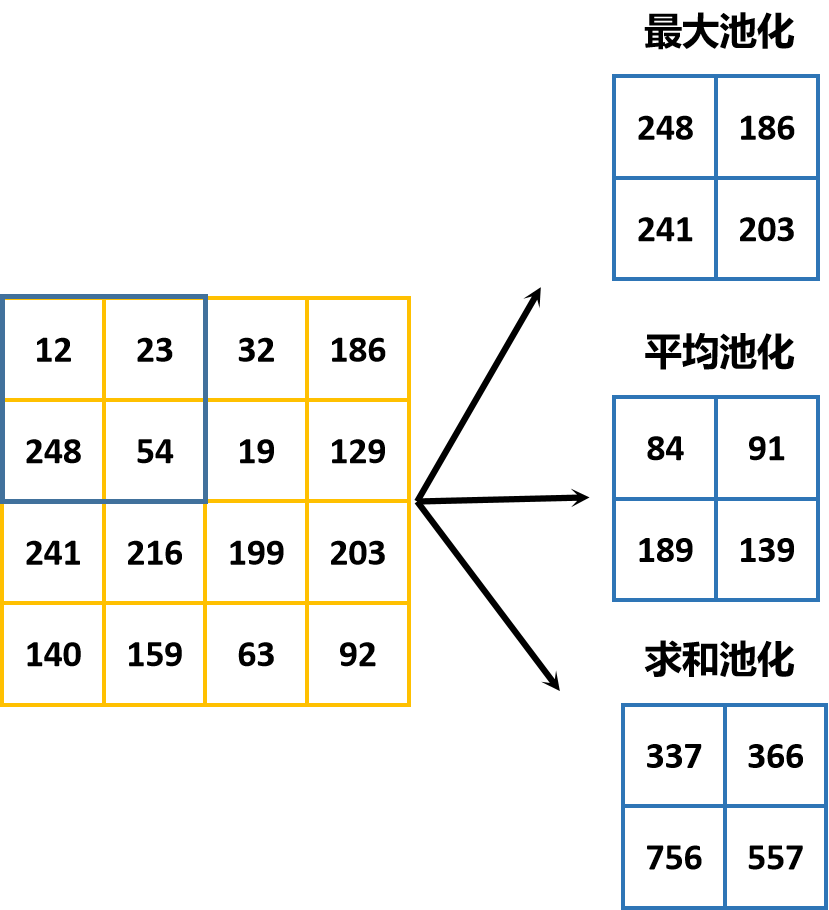
\includegraphics[width=0.5\textwidth]{figures/pooling.png}
	\caption{最大池化,平均池化和求和池化的运算方式。}
	\label{pooling}
\end{figure}

图\ref{pooling}展示了三种不同类别池化操做的计算过程。与卷积核的计算方式大体相同,同样的是从特征图的左上角像素区域依次移动到特征图的右下角。与卷积核一样,池化层的步长也是可以设置的。通常情况下,两个或三个像素窗口大小步长为2的池化层被证明具有良好的效果。最大池化会提取像素区域内像素值最大的作为输出,求和池化会将像素区域内的所有像素值求和后输出,平均池化则是在对像素区域内的所有像素值求和之后取平均值再输出。值得注意的是,不论是哪种类型的池化操做,特征图的大小都缩小为原始尺寸的一半。特征图的缩小,并不会影响卷积神经网络的精度,因为池化操做提取出每个窗口像素区域内最主要的特征,这意味着卷积神经网络可以不太关心特征的在原始特征图的确切位置,只要某个特征能够匹配窗口中的特征。换句话说,这样做的结果是卷积神经网络可以发现某个特征是否在图像中,而不必关心这个特征在输入图像中的具体位置。

从功能上来讲,最大池化主要用于\textbf{噪声抑制(Noise Suppressant)}。因为它完全抛弃像素区域内其他值,只保留最大像素值。然而,平均池化和求和池化却仍然保留像素区域内的所有像素值,这会使得像素区域内的噪声也会被融合进主要特征中。在实践中,最大池化的平均性能要优于平均池化和求和池化。综上,池化的主要作用有以下:

\begin{itemize}
	%\vspace{-1em}
	\item 减少特征图维度,从而减少计算量和模型的参数量;
	\item 消除输入图像中的小变换、扭曲和平移对卷积神经网络的影响,因为这些因素不会改变池化层的输出结果;
	\item 让卷积神经网络可以发现输入图像中任意位置的特征;
\end{itemize}

\subsection{全连接层}
在卷积神经网络分类图片的最后一步,是使用一个分类器对前置网络层提取出来的特征进行投票分类。因此,在卷积神经网络的最后一层都是一个分类器,这个分类器可以使用其他分类器如SVM等。但一般为了保证神经网络是可以端到端训练的,通常都会使用\textbf{全连接层} 来作为最后结果的分类器。全连接层是一个传统的多层感知器,全连接层中的每一个神经元都彼此相互连接,使用eq.\ref{softmax} softmax作为激活函数。softmax函数是逻辑函数的一种推广,它可以将一个含任意实数的K维向量z,映射到另一个K维向量$\sigma (Z)$中,并且所有元素之和为1。因此,softmax被广泛用于基于概率的多分类问题中。以输入向量[1,2,3,4,5,6,7]为例,该向量经过softmax输出后的结果为[0.002, 0.004, 0.012, 0.032, 0.086, 0.233, 0.633]。输出向量中拥有最大权重的项对应着输入向量中的最大值7。这表明了该函数的作用:对向量进行归一化,凸显其中最大的值并抑制远低于最大值的其他分量。

\begin{equation}
\begin{aligned}
\label{softmax}
\sigma (Z)_j = \frac{e^{z_j}}{\sum_{k=1}^N e^{z_k}}  (j=1....K)
\end{aligned}
\end{equation}

图\ref{fclayer}展示了全连接层是如何对卷积层和池层的输出表示输入图像的高级特征进行分类判别的。在该图示例中,输入的原始图像数据,在经过多个卷积+relu+池化层之后,最终输出了两个特征图,这些特征图中蕴含了图像的高级特征。将这些特征图进行\textbf{flatten}操做后,便能将二维的特征图变换成一维的输入向量,输入到全连接层中进行运算。使用上述提到的softmax激活函数,即可以将这个一维向量映射到最后的输出向量。输出向量的输出内容[p1,p2,p3,p4],即表示了该输入图像的类别可能性。在该示例中,全连接层是一个四分类器。在实践中,几个全连接层通常叠加在一起,中间的层被称做 \textbf{隐层(hidden layer)},每增加一层,网络就可以学习到更复杂的功能组合,做出更好的类别预测。

\begin{figure}[ht]
	\centering
	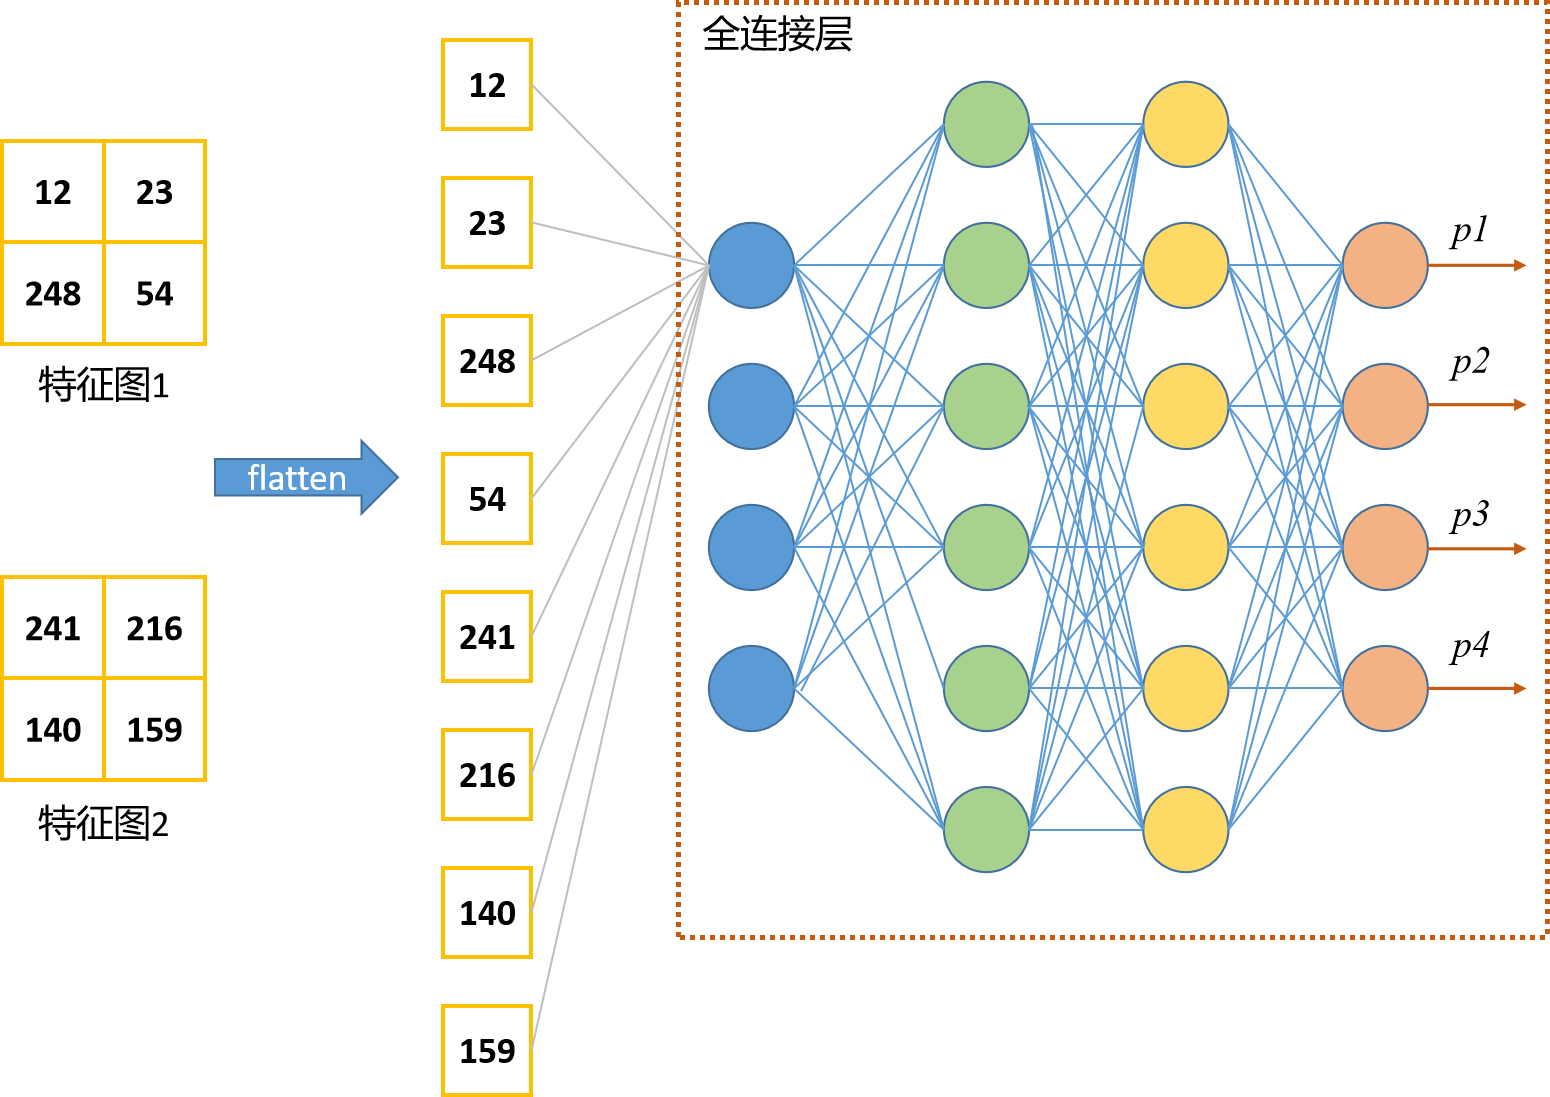
\includegraphics[width=0.8\textwidth]{figures/fclayer.png}
	\caption{全连接层。}
	\label{fclayer}
\end{figure}

\subsection{整体架构}
图\ref{framework}展示了一个完整卷积神经网络的架构和其实际推理计算的结果。图中的conv表示卷积核层,relu表示非线性激活层,pool表示池化层,fc表示全连接层。图中直观清楚的展示了图片经过每一层后的输出效果。可以看到在经过前几层卷积核的运算之后,特征图将小狗的大致轮廓提取了出来。在后面几层卷积核中,提取了小狗更细致的细节特征。值得注意的是,在最后的分类结果中,这张图片被分类为了马,马有着最高的置信度。之所以出现这样的结果可能是来自于这张小狗的轮廓外形和站立的马十分相似,在卷积神经网络的前几层提取出来的全都是外形特征。在后面几层卷积核的处理中虽然提取了这张图片的细节,最后全连接层在分类时稍微让小狗类别的置信度增加了一点,但是根据卷积网络前面几层的主要结果,这张图片仍然被分类为了马。这个例子也从侧面说明了,为什么加深网络能够带来图片分类精度的提升。若在这个例子上加深该卷积神经网络,随着后续网络层抽取更多图片的细节特征,或许这张图片的分类结果的小狗置信度反倒会上升超过马,使得最终的分类结果为小狗。

另一个值得注意的是,每一个卷积核的后面都有一个relu层,就如上文中的提到的那样,它既不改变图片尺寸大小也不改变特征图内容,只是让主要特征更凸显出来。如图\ref{framework}所示,每一个relu层输出内容都让卷积运算的结果更明显,以方便后一次卷积运算。总的来说,卷积层数越多,卷积网络就能够学会识别越复杂的特征。
\begin{figure}[ht]
	\centering
	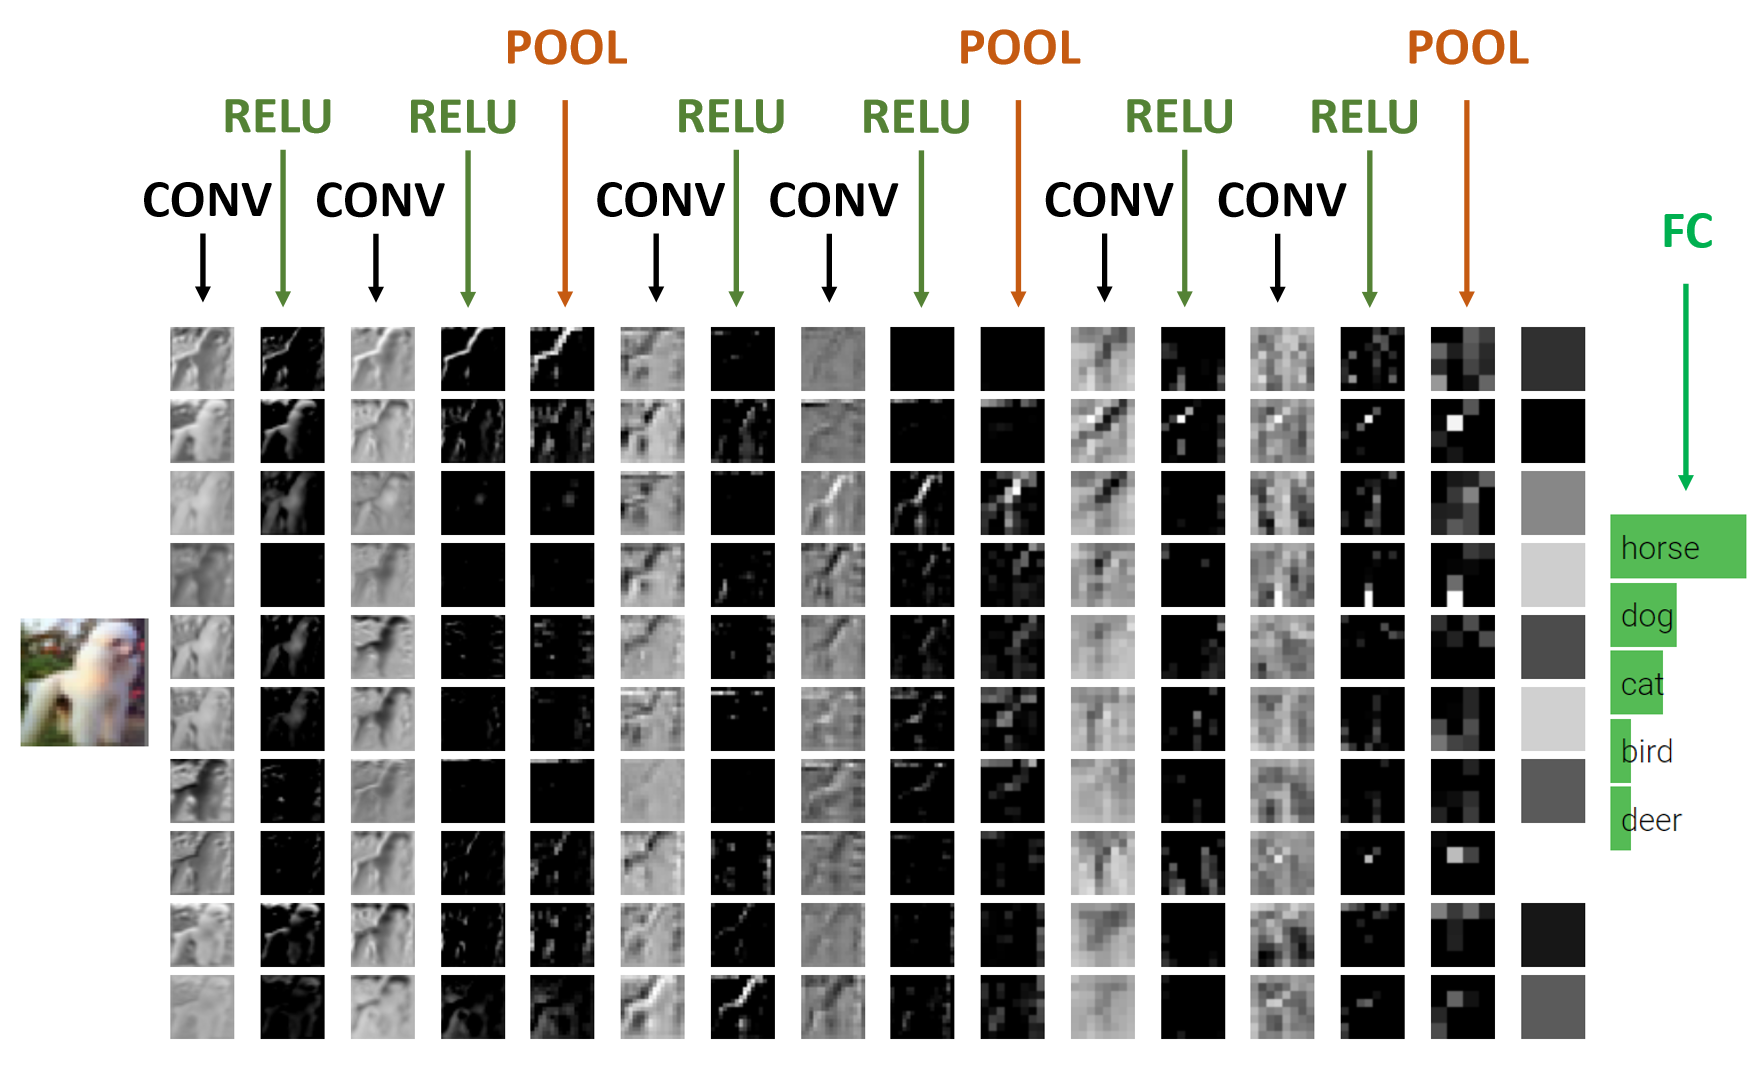
\includegraphics[width=1\textwidth]{figures/vggResult.png}
	\caption{vgg16的整体架构和在cifar10数据集上的计算结果。}
	\label{framework}
\end{figure}

\section{数据集}

在本节中,将介绍本文实验中使用的不同数据集。本文使用多种数据及进行各种机器学习任务,用以测试提出的模型压缩和优化方案的性能。实验中使用的数据集包括用于图像分类的MNIST、Cifar-10和ImageNet。

\begin{figure}[]
    \centering
    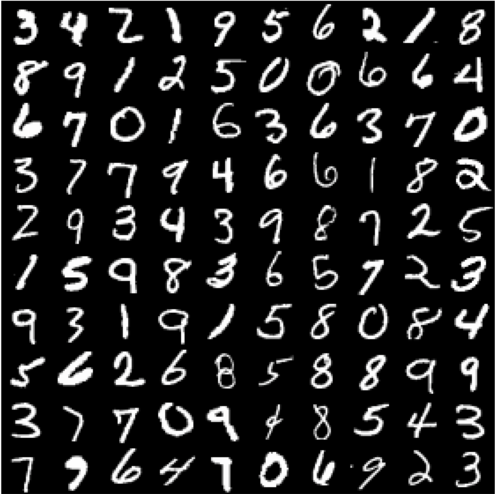
\includegraphics[width=0.8\textwidth]{mnist.png}	%\vspace{-1.0em}
    \caption{MNIST}
    \label{fig:mnist} %\vspace{-0.8em}
\end{figure}

\begin{figure}[]
    \centering
    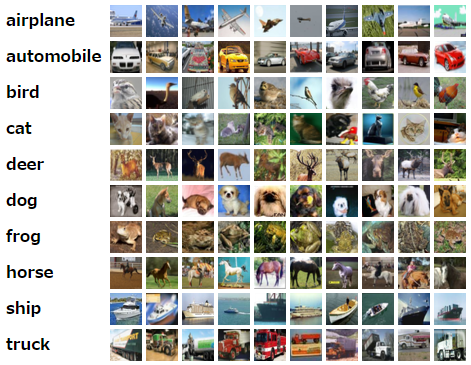
\includegraphics[width=0.8\textwidth]{cifar10.png}	%\vspace{-1.0em}
    \caption{Cifar-10}
    \label{fig:cifar10} %\vspace{-0.8em}
\end{figure}

\begin{figure}[]
    \centering
    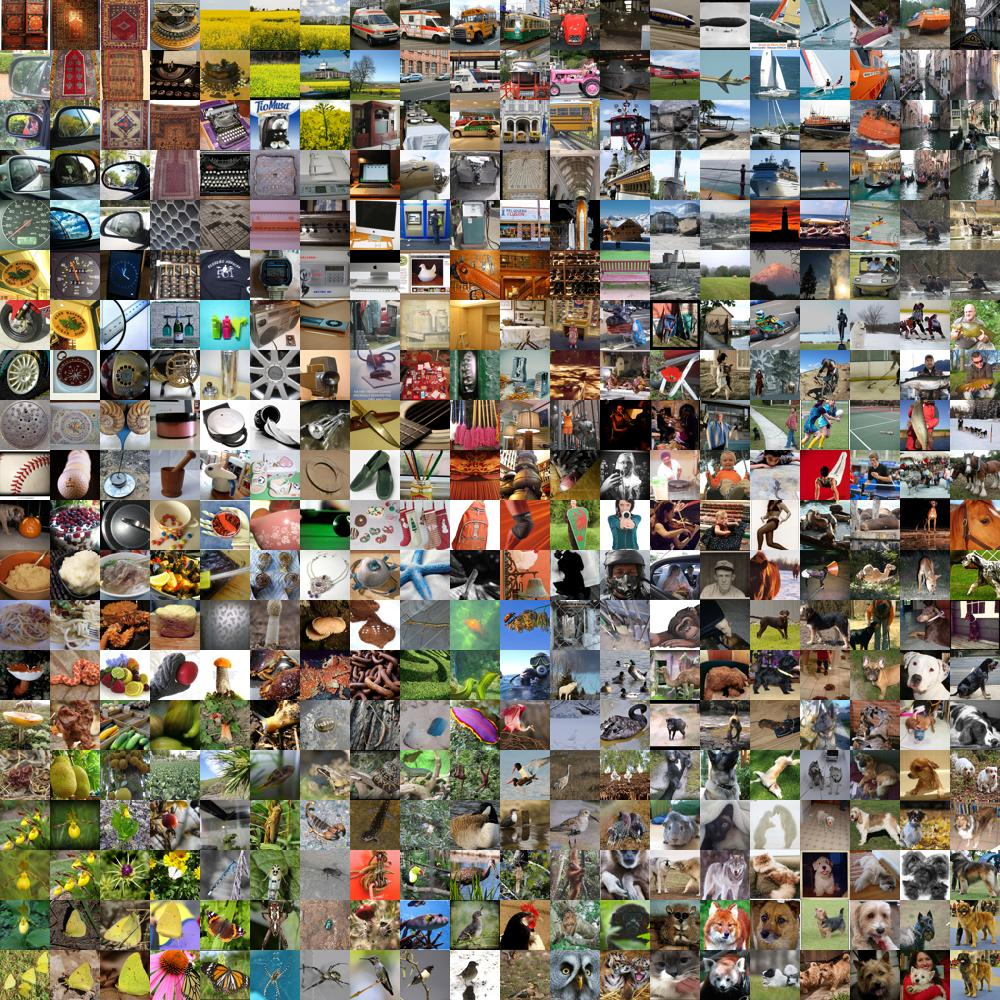
\includegraphics[width=1\textwidth]{imagenet.jpg}	%\vspace{-1.0em}
    \caption{ImageNet}
    \label{fig:imagenet} %\vspace{-0.8em}
\end{figure}

\begin{itemize}
    \item MNIST: 如图~\ref{fig:mnist}所示,MNIST数据集(Mixed National Institute of Standards and Technology database)是美国国家标准与技术研究院收集整理的大型手写数字数据库[lecun1998mnist],用于进行手写数字识别,一共10各类表示10个数字,图片大小为28*28,一共包含60,000个示例的训练集以及10,000个示例的测试集。这个数据集相对来说比较简单和小,只需要几分钟的时间来训练模型。我们只使用MNIST进行原型设计,并使用更大的数据集进一步验证每个想法。
    \item CIFAR-10: 如图~\ref{fig:cifar10}所示,CIFAR-10数据集由60000个32x32彩色图像组成,其中有50000个训练图像和10000个测试图像,包含互不相关的10个类\cite{krizhevsky2009learning},每个类都有6000个图像示例,。数据集比MNIST稍难一些,但模型仍然只需要几个小时的训练。当需要多次重复一组类似的实验时,我们使用Cifar-10进行消融研究。
    \item ImageNet:如图~\ref{fig:imagenet}所示,ImageNet是一个针对ILSVRC挑战的大规模数据集\cite{krizhevsky2012imagenet}。其中,训练数据集包含1000个类别和120万幅图像,验证数据集包含50,000张图像,每个类50张。使用Top1和Top5的准确率表示分类性能的结果,Top1准确率衡量的比例正确标记的图像,而Top5表示如果五个概率最大的标签中有一个是正确的标签,那么这张图像就被认为是一个正确的标签。我们使用ImageNet数据集来测量模型压缩和优化的性能。
\end{itemize}

%\section{实验环境说明}
%
%\subsection{深度学习框架说明}
%
%直接编程一个多核CPU或GPU程序是比较困难的,但幸运的是,目前深度学习相关开源框架的生态非常完美,国内外都有多个开源框架习供研究者和开发者使用,光是为人熟知的就有Caffe,Tensorflow,Pytorch,Keras,Mxnet,NCNN等,它们将神经网络的计算抽象成一些基本的操作,如卷积,矩阵乘法等,并进行高度优化。用户只需要关注高级神经网络架构而不是低级实现,因此程序员只需要写一个计算描述,然后深度学习框架就可以高效地将计算映射到高性能硬件上。在本文中,主要是通过Pytorch对神经网络进行训练和验证,使用NCNN和TensorRT在嵌入式平台上进行部署和推理验证。
%
%\begin{itemize}
%    \item Pytorch: PyTorch\cite{pytorch}是有Facebook推出的一个最新的、更灵活的深度学习框架,专门针对 GPU 加速的深度神经网络(DNN)编程,支持动态图。我们使用PyTorch进行了网络模型的训练和压缩优化算法实现。
%    \item NCNN: NCNN \cite{ncnn} 是一个为嵌入式设备极致优化的高性能神经网络推理框架,只支持部署和推理。我们使用NCNN将网络模型部署到嵌入式设备上查看资源使用情况和性能测试。
%    \item TensorRT: TensorRT \cite{tensorrt} 是NVIDIA的一款高性能深度学习推理框架,包含深度学习推理优化器和运行环境,可为深度学习推理应用提供低延迟和高吞吐量。我们使用NCNN将网络模型部署到嵌入式设备上查看资源使用情况和性能测试。
%\end{itemize}
%
%\section{模型压缩与优化方法}
%
%近年来,深层卷积神经网络(CNN)因为其强大的表示能力,越来越广泛应用于各个领域。并且随着CNN的巨大成功,在实际应用中部署深度网络的需求不断增加。但巨大的计算复杂性在实际应用中的CNN部署中引入了两个问题。一种是随着计算复杂度的增加,CNN推理阶段变慢。这使得很难在实时应用程序中部署CNN。另一个问题是,CNN固有的密集计算将消耗大量的电池电量,而这仅限于移动设备。同时,CNN的大量参数会消耗相当多的存储空间和运行时内存,而这在嵌入式设备上是非常有限的。因此,减少CNN的存储和计算成本变得至关重要,网络的优化和加速已经成为目前深度学习研究的一个热门话题。
%
%近年来深度神经网络压缩和加速领域的研究取得多方面的进展。根据它们的性质,我们将这些优化方法分为五类:模型修剪、矩阵/张量分解、模型参数量化、高效网络设计。这些方法大多数是相互正交且相互补充的,可以同时应用。比如说,为了达到更高的压缩比,高效卷积网络和参数修剪与量化可以一起部署。同样的,模型量化也可以与低秩分解一起使用,以实现更好的压缩和加速效果。我们将在以下各节中分别描述它们的详细特性以及优点和缺点的分析。
%
%
%\subsection{模型修剪}
%
%早期的剪枝研究最佳脑损伤\cite{lecun1989optimal}和最佳脑外科\cite{denil2013predicting}方法基于损失函数的黑森性减少了连接数。他们的研究表明,这种剪枝比基于大小的剪枝(如重量衰减法)具有更高的准确性。
%
%在这个研究方向上,后面的趋势是在预先训练好的DNN模型中修剪冗余的、无信息的权重。如Srinivas和Babu\cite{srinivas2015data}对神经元之间的冗余进行了研究,提出了一种去除冗余神经元的无数据剪枝方法。Han等人\cite{han2015learning}提出减少整个网络的参数总数和操作总数。Chen等人\cite{chen2015compressing}提出了一种哈希网模型,该模型使用低成本哈希函数将权重分组到哈希桶中以共享参数。\cite{han2015deep}中的深度压缩方法去除冗余连接并对权重进行量化,然后利用Huffman编码对量化后的权重进行编码。在\cite{ullrich2017soft}中,提出了一种基于软权重共享的简单正则化方法,将量化和修剪都包含在一个简单的(再)训练过程中。上述剪枝方案通常在DNNs中产生连接剪枝。
%
%人们对训练具有稀疏性约束的紧凑DNN也越来越感兴趣。这些稀疏性约束通常作为低范数或L1范数正则化引入优化问题中。\cite{lebedev2016fast}中的工作对卷积滤波器施加了组稀疏性约束,以实现结构性脑损伤,即以组方式对卷积核的条目进行修剪。在\cite{zhou2016less}中,在训练阶段在神经元上引入了一组稀疏正则化器来学习具有简化滤波器的紧凑CNN。Wen等人\cite{wen2016learning}为了减少冗余的滤波器、通道甚至层,在网络的每一层上增加了一个正则化器来引导结构化稀疏。在层级剪枝中,以上所有的工作都使用了L2范数正则化器。\cite{li2016pruning}中的作品使用L1-Norm来选择和修剪不重要的过滤器。
%
%值得注意的是,使用网络修剪的需要注意一些问题。首先,相对来说,使用L2正则化来进行剪枝更加难以收敛,往往需要更多次的迭代;此外,所有的修剪条件都需要手动对参数进行微调,设置层的敏感性,对于一些应用程序来说可能会比较麻烦;最后,网络剪枝通常能够减少模型规模,但不能显著提高效率(训练或推理时间)。
%
%\subsection{矩阵/张量分解}
%
%利用低秩分解来加速卷积已经有很长一段时间了,例如,高维离散余弦变换(DCT)和由一维DCT变换和一维小波分别构造张量积的小波系统。Rigamonti等人\cite{rigamonti2013learning}用字典学习的方法介绍了学习可分离1D滤波器。对于一些简单的网络模型,在\cite{denton2014exploiting}中使用了一些卷积核的低秩近似和聚类方案仅仅付出分类精度下降1 \% 的微小代价就实现单个卷积层上的2倍加速。\cite{jaderberg2014speeding}的工作提出了使用不同的张量分解方案,在文本识别的工作中仅仅损失1 \% 的准确性的前提下得到了 4.5×的速度提升。
%
%经典的压缩3D卷积层的方法通常是低秩近似逐层进行,完成后固定一层的参数,并根据重构误差准则对以上各层进行微调,如图~\ref{fig:low-rank}所示。在此基础上,\cite{lebedev2014speeding}使用非线性最小二乘来计算CP分解对核张量进行了正则多元分解。\cite{tai2015convolutional}则提出了一种新的低秩张量分解算法,它使用批处理标准化(BN)来转换内部隐藏单元的激活,用于从零开始训练低秩约束CNN。一般来说,\cite{tai2015convolutional}(BN低秩)中的CP和BN分解方案都可以从零开始训练CNN。然而,它们之间几乎没有什么区别。例如,在CP分解中寻找最佳低秩近似是一个不适定问题,因为最佳K秩数近似有时可能不存在。而对于BN格式,分解总是存在的。如表~\ref{tab:low-rank}所示,本文对这两种方法进行了简单比较,通过实际的加速比和压缩率来衡量他们的性能。
%
%\begin{figure}[]
%    \centering
%    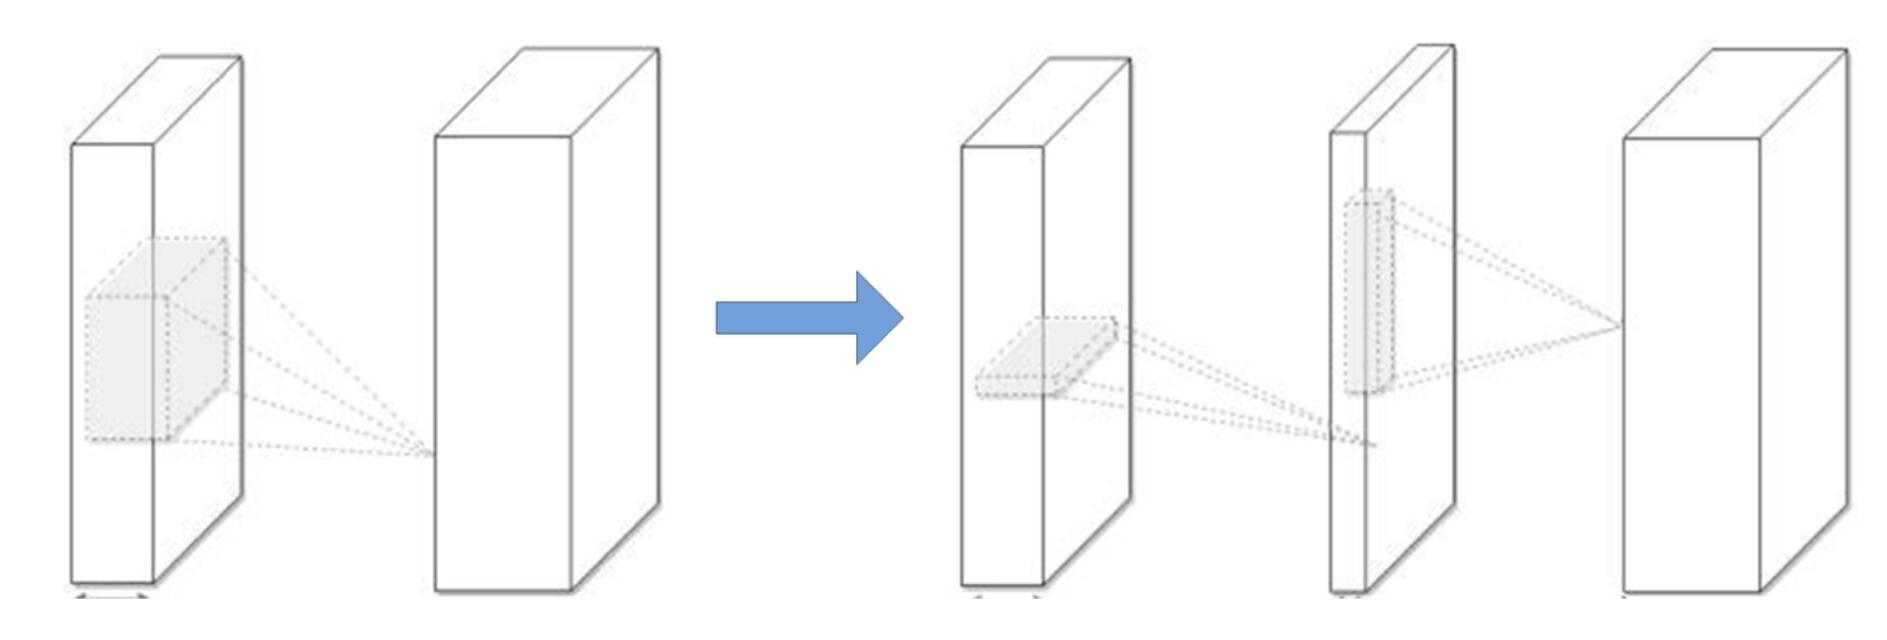
\includegraphics[width=0.8\textwidth]{low-rank.jpg}	%\vspace{-1.0em}
%    \caption{低秩正则化方法的一个典型框架。左边是原卷积层,右边是秩为k的低秩约束卷积层}
%    \label{fig:low-rank} %\vspace{-0.8em}
%\end{figure}
%
%\begin{table}[]
%    \centering
%    \caption{ILSVRC-2012上不同低秩模型及其基线的比较}
%    \label{tab:low-rank} %\vspace{-0.8em}
%    \begin{tabular}{llll}
%    模型          & Top-5 准确率 & 加速比  & 压缩率  \\ \hline
%    AlexNet     & 80.03\%   & 1.   & 1.   \\
%    BN Low-rank & 80.56\%   & 1.09 & 4.94 \\
%    CP Low-rank & 79.66\%   & 1.82 & 5.   \\ \hline
%    VGG-16      & 90.60\%   & 1.   & 1.   \\
%    BN Low-rank & 90.47\%   & 1.53 & 2.72 \\
%    CP Low-rank & 90.31\%   & 2.05 & 2.75 \\ \hline
%    GoogleNet   & 92.21\%   & 1.   & 1.   \\
%    BN Low-rank & 91.88\%   & 1.08 & 2.79 \\
%    CP Low-rank & 91.79\%   & 1.20 & 2.84 \\ \hline
%    \end{tabular}
%\end{table}
%
%值得注意的是,虽然基于低秩近似的矩阵分解方法可以直接用于模型压缩和加速,但是因为它涉及到分解操作,具有较高的计算复杂度,并不容易有高效实现;同时,鉴于不同的层包含不同的信息不能进行全局参数压缩,目前的方法是逐层进行低秩近似;最后,因式分解后得模型需要较多的重训以达到与原始模型相比的准确度。
%
%
%\subsection{参数量化}
%
%网络参数量化通过减少表示每个权值所需的比特数来压缩原始网络。Gong等人的\cite{gong2014compressing}和Wu等人的\cite{wu2016quantized}对参数值进行k-means标量量化。Vanhoucke等人\cite{vanhoucke2011improving}表明,参数的8位量化可以在精度损失最小的情况下导致显著的加速。\cite{gupta2015deep}在基于随机四舍五入的CNN训练中使用了16位定点表示,显著减少了内存使用量和浮点运算,分类精度几乎没有损失。
%
%\begin{figure}[]
%    \centering
%    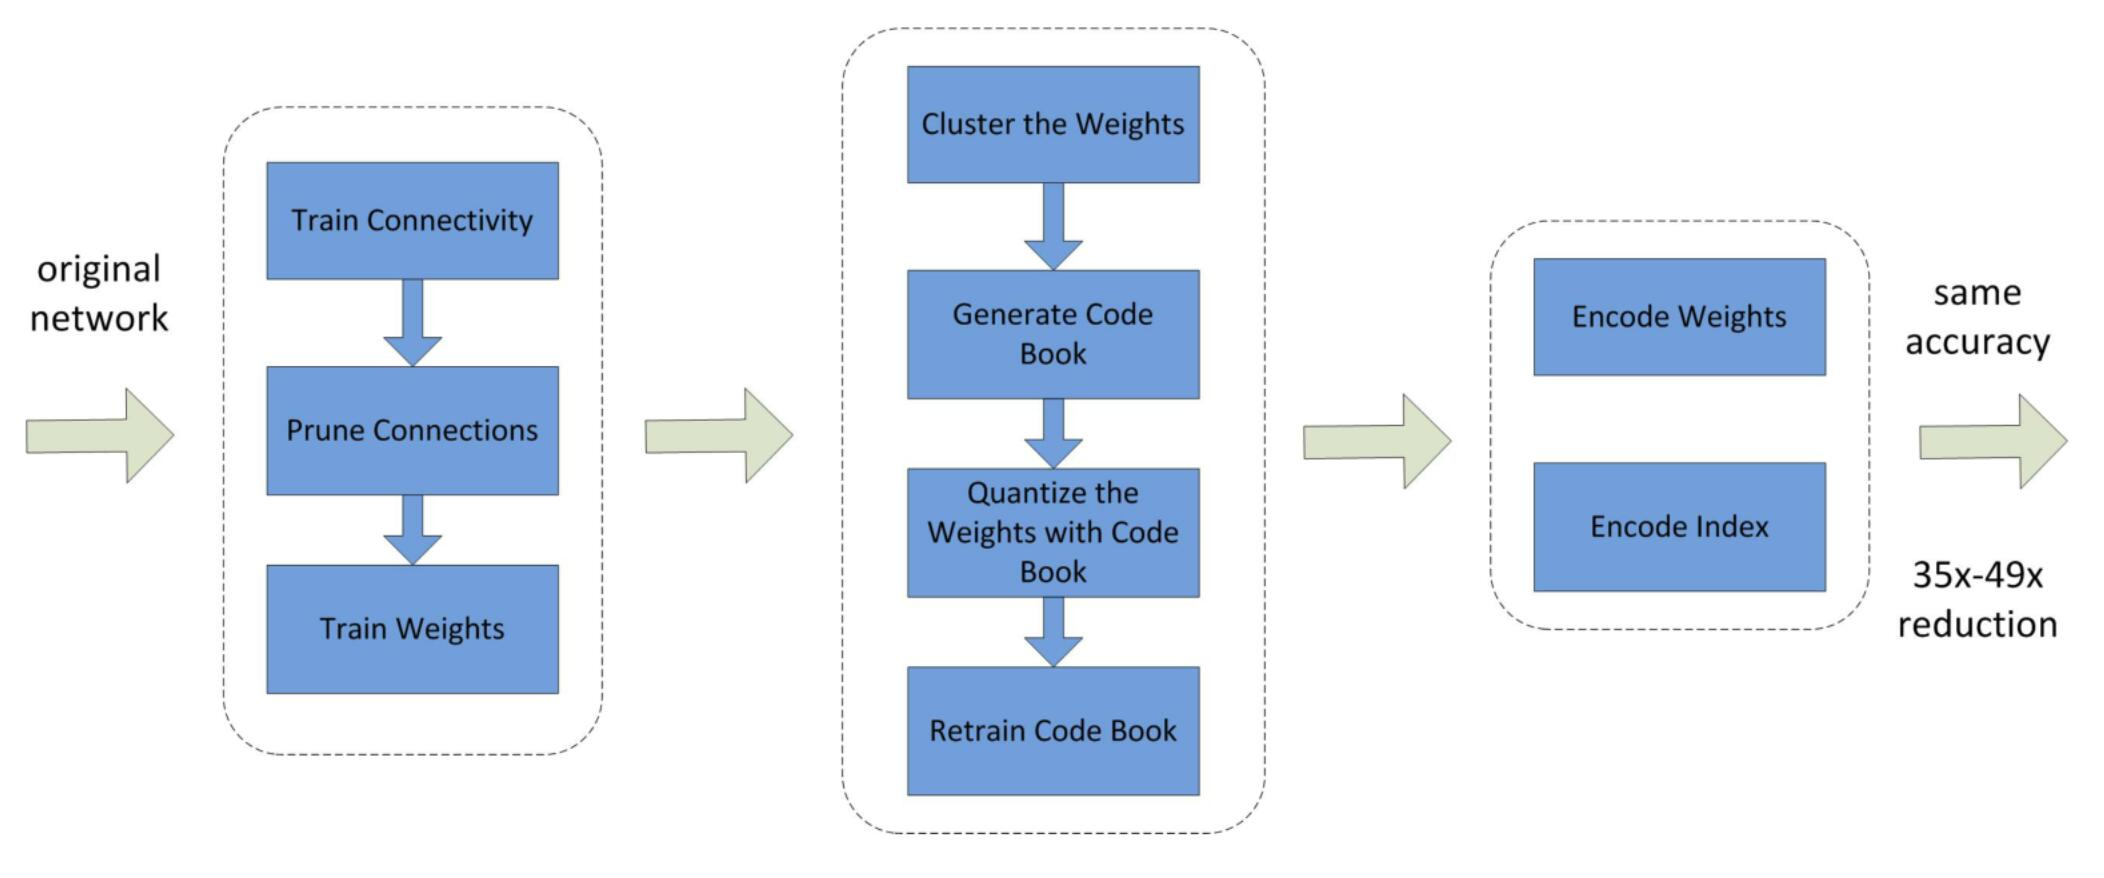
\includegraphics[width=0.8\textwidth]{han-compress.jpg}	%\vspace{-1.0em}
%    \caption{Han提出的三阶段压缩方法:剪枝、量化和huffman编码。输入是原始模型,输出是压缩后的模型。}
%    \label{fig:han-compress} %\vspace{-0.8em}
%\end{figure}
%
%\cite{han2015deep}中提出的方法采用权值共享的方式对连接权值进行量化,然后对量化后的权值和码本进行Huffman编码,进一步降低速率。如图~\ref{fig:han-compress}所示,它首先通过正常的网络训练学习连接,然后修剪小权重连接。最后,对网络进行再训练微调,以恢复网络模型的能力与精度。在所有基于量化的方法中,这项工作达到了最先进的性能。在\cite{choi2016towards}中,证明了使用Hessian权值可以度量网络参数的重要性,并提出了最小化Hessian权值对聚类参数的平均量化误差。
%
%量化是一种非常有效的模型压缩和加速方法。在极端情况下,甚至可以使用1位表示每个权重的值,即二进制权值神经网络,采用01来表示模型的权重参数和激活值。有几种方法可以直接用二进制权值训练卷积神经网络,例如BinaryConnect\cite{courbariaux2015binaryconnect}, BinaryNet\cite{courbariaux2016binarized}和XNOR\cite{rastegari2016xnor}。\cite{merolla2016deep}的一项系统研究表明,使用反向传播训练可以恢复量化网络(包括二进制权值)的性能。
%
%但是,二进制网络的准确性在面对GoogleNet这样的大型网络时显著降低。同时,现有的二值化方案基于简单的矩阵近似,表达能力不够,精度的损失较大。为了解决这个问题,在\cite{hou2016loss}的工作提出了一个近牛顿算法与对角Hessian近似,直接最大限度地减少与二进制权值有关的损失。\cite{lin2015neural}通过随机二值化权值,将隐藏状态计算中的乘法转化为显著变化,减少了训练阶段浮点乘法运算的时间。Zhao等人提出了半波高斯量化来学习低精度网络,取得了令人满意的结果。
%
%\subsection{高效网络设计}
%
%卷积网络加速和压缩的目标是优化给定深度神经网络的执行和存储框架,对网络加速和压缩的另一个平行探索是设计更高效但低成本的网络架构本身。
%
%在\cite{lin2013network}中,作者提出了NIN架构,使用1x1卷积在保持整体计算复杂度较小的前提下来增加网络容量,为了减少CNN模型的存储需求,他们还提出去除完全连接层,并使用全局平均池。这些策略也被许多最先进的CNN模型使用,如GoogleNet\cite{szegedy2015going}和ResNet\cite{he2016deep}。分组卷积是降低网络复杂度的另一种常用策略,GoogleNet\cite{szegedy2015going}的研究中也探讨了这一点。\cite{iandola2016squeezenet}中提出的SqueezeNet通过大量使用1 × 1卷积和分支策略,在于AlexNet精度相当的前提下实现了约50倍的参数压缩。通过分支结构,\cite{xie2017aggregated}的ResNeXt工作可以在相同的计算预算下获得比ResNet更高的精度。MobileNet\cite{howard2017mobilenets}中提出的深度可分离卷积将分组卷积发挥到极致,即分组的数量等于输入/输出通道的数量,由此产生的MobileNet可以比VGG16模型小32倍,快27倍,它们在ImageNet上具有相似的图像分类精度。文献\cite{zhang2018shufflenet}中提出的shuffle网引入了信道shuffle操作,增加了多组内的信息变化,显著提高了网络的表示能力。他们的方法在AlexNet上实现了大约13倍的实际加速,而且精度相当。
%
%然而手动设计高效模型仍然是一项挑战,因为要考虑太多因素且需要研究人员大量的相关经验和知识。因此另一个研究致力于使用启发式和基于规则的策略进行自动的网络架构搜索\cite{zoph2016neural}。
%
%\subsection{知识蒸馏}
%
%最早利用知识转移(knowledge transfer,KT)来压缩模型的是由Caruana等人\cite{buciluǎ2006model}提出的,他们使用一个大网络的输出来训练了一个带有伪数据标记的强分类器压缩/集成模型,但这项工作仅限于肤浅的模型。这个想法最近在\cite{ba2013deep}中被采用,将使用复杂模型指导和训练简单模型的方法乘坐知识蒸馏(knowledge distillation,KD),基于KD方法的主要思想是通过柔性标签分布输出,将知识从大型教师网络模型转换为小型学生网络模型。
%
%\cite{hinton2015distilling}的工作提出了KD压缩框架,它通过遵循学生-教师范式来简化深度网络的训练,在这种范式中,学生根据教师输出的柔性标签进行惩罚。该框架将教师网络压缩成深度相似的学生网络。训练学生预测输出和分类标签。尽管它很简单,KD在各种图像分类任务中展示了有希望的结果。\cite{romero2014fitnets}的提出了一种利用深度神经网络来解决网络压缩问题的方法,称为FitNets,通过训练一个薄而深的网络来压缩宽而浅(但仍然深)的网络。该方法扩展了思想,允许更薄和更深的学生模型。为了从教师网络的中间表示中学习,FitNet让学生模拟教师的全部特征图。然而,这样的假设太严格了,因为老师和学生的能力可能有很大的不同。
%
%沿着这个方向,蒸馏知识有几个扩展。\cite{korattikara2015bayesian}的工作是通过蒙特卡洛近似法来用一个预训练的教师模型训练学生模型。所提出的框架使用在线训练,并使用深度神经网络的学生模型。不同于以往的用柔标概率表示知识的工作,\cite{luo2016face}是利用较高隐层的神经元来表示知识,它保留了与标签概率一样多的信息,但更加紧凑。\cite{chen2015net2net}的工作通过瞬间将知识从以前的网络转移到每一个新的更深或更宽的网络,加速了实验过程。这些技术是基于神经网络规范之间的函数保持变换的概念。Zagoruyko等人\cite{zagoruyko2016paying}提出注意转移(AT)来放宽FitNet的假设。
%
%值得注意的是,基于KD的方法虽然可以使更深层次的模型变 得更浅,并帮助显著降低计算成本,但是也有一些缺点。其中之一是KD的应用有局限性,只能应用于以softmax为损失函数的任务;另一个缺点是,与其他类型的方法相比,基于KD的方法的压缩性能并不突出。

\section{本章小结}

在本章,我们介绍了论文的实验环境,也重点介绍了深度学习与模型压缩加速的基本理论知识。首先引入了机器学习领域中发展最为迅速的研究方向——深度学习,介绍其原理;然后从五个方面介绍了深度神经网络的压缩与优化方法,并对其优点与缺点进行了讨论和分析。本章旨在为读者提供一个本文工作的背景知识,为读者建立对深度学习和卷积神经网络的整体概念,同时对深度神经网络模型压缩与优化领域的研究做个基础的理论铺垫,以便读者更好地理解后面章节的研究和实验工作。